\section{Resultados}

\begin{frame}
  \frametitle{}
%  \begin{table}
%   \input{../../outputs/tabela_descritiva_com_harmatan.tex}
%  \end{table}
   Diretrizes da Organização Mundial de Saúde (OMS):
  \begin{itemize}
    \item Média diária $MP_{2.5}$: só 1\% dos dias pode ultrapassar 25 $ug/m^3$;
    \item Média anual $MP_{2.5}$: 10 $ug/m^3$;
    \item Média diária $MP_{10}$: só 1\%  pode ultrapassar 50 $ug/m^3$;
    \item Média anual $MP_{10}$: 20 $ug/m^3$.
  \end{itemize}
\end{frame}

\begin{frame}
  \frametitle{}
  \begin{figure}[H]
    \centering
    \includegraphics[width=0.5\textwidth]{../../outputs/windRose2007.pdf}
    \caption{Rosa do ventos para Acra/2007. \label{fg:rosaCompleta}}
  \end{figure}
\end{frame}


\begin{frame}
  \frametitle{}
  \begin{figure}[H]
    \centering
    \includegraphics[width=0.8\linewidth]{../../outputs/windRose_horaria.pdf}
    \caption{Rosa do ventos horária para Acra/2007. \label{fig:windRose_horaria}}
  \end{figure}
\end{frame}


\begin{frame}
  \frametitle{}
  \begin{figure}[H]
    \centering
    \includegraphics[width=0.8\linewidth]{../../outputs/windRose_mensal.pdf}
    \caption{Rosa do ventos mensal para Acra/2007. \label{fig:windRose_mensal}}
  \end{figure}
\end{frame}



\begin{frame}
  \frametitle{}
  \begin{figure}[H]
    \centering
    \begin{subfigure}[b]{0.5\linewidth}
      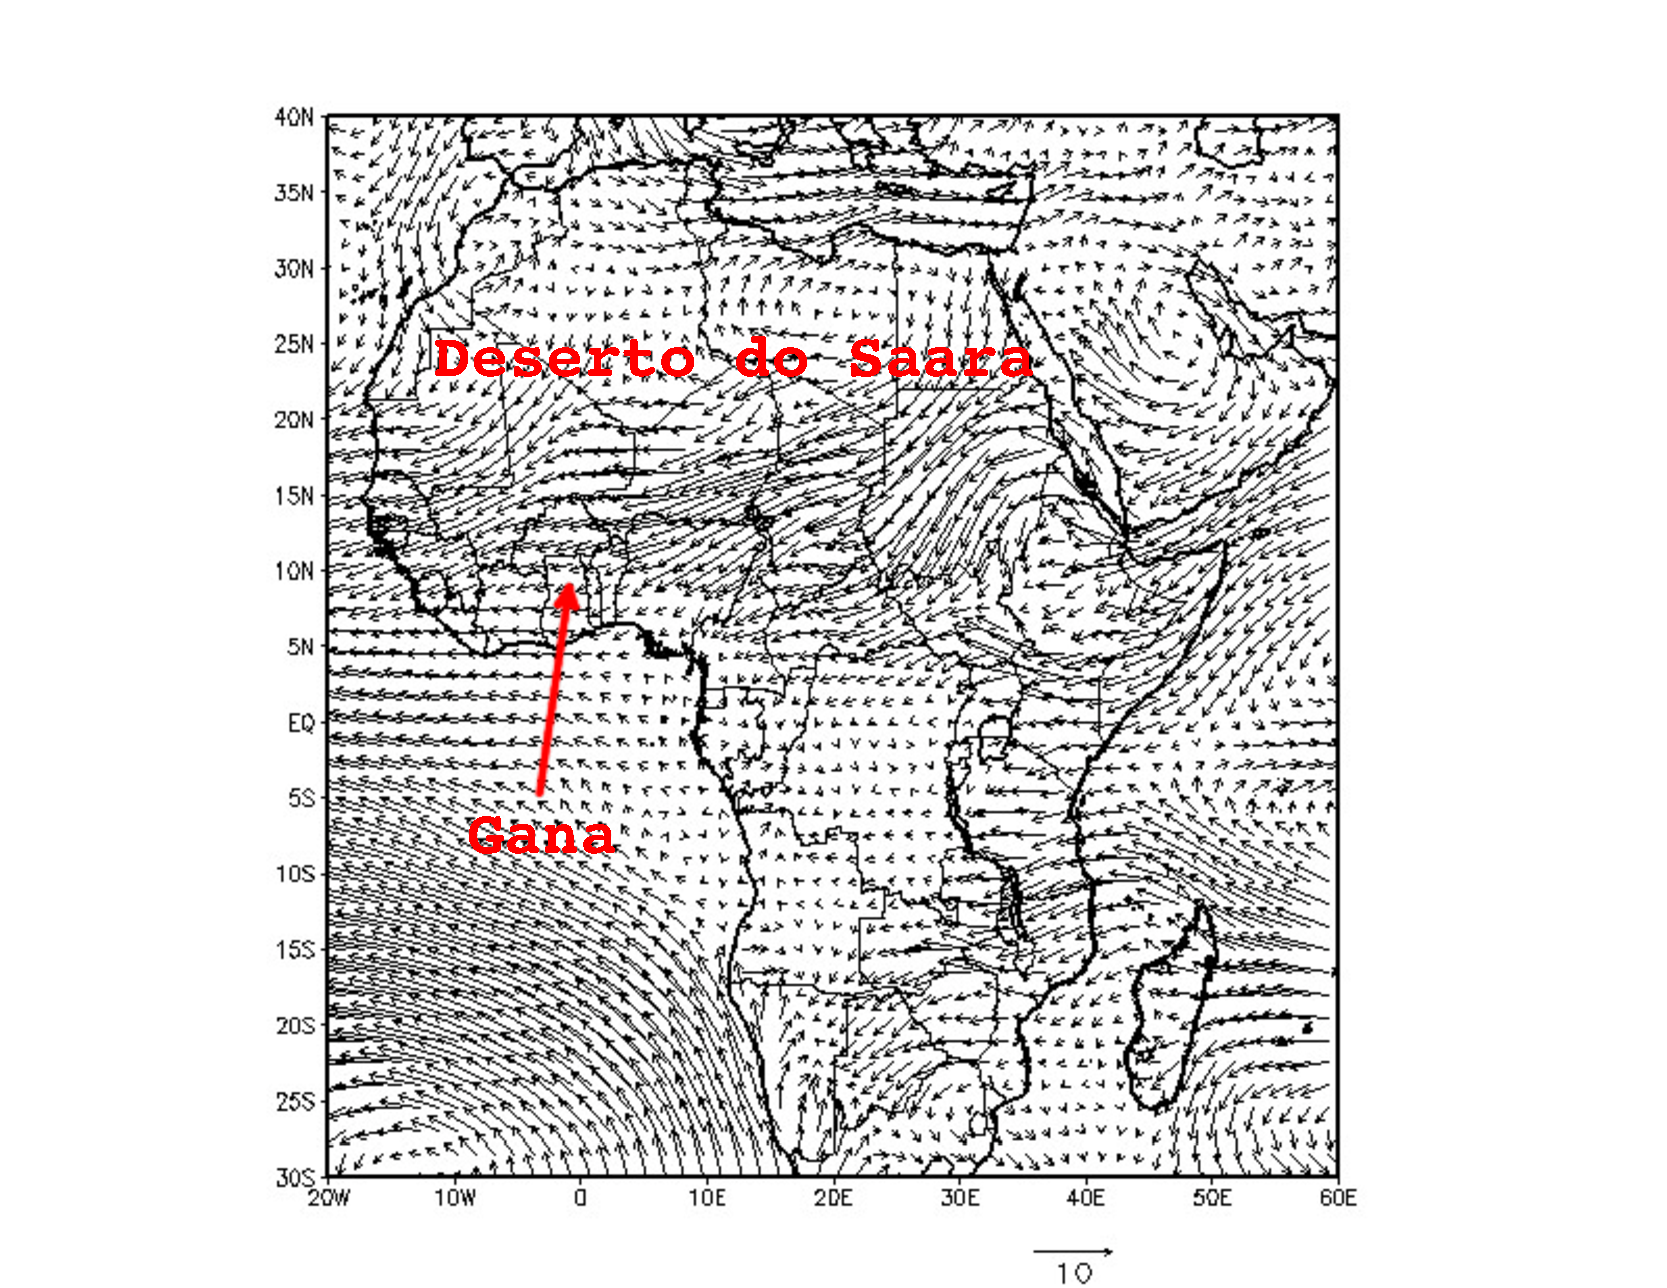
\includegraphics[width=\linewidth]{../../inputs/grads/gimp/875hPa/DEZ_2007.pdf}
      \caption{Dezembro de 2007}
    \end{subfigure}%
  %  \hspace{0.5cm}
    \begin{subfigure}[b]{0.5\linewidth}
      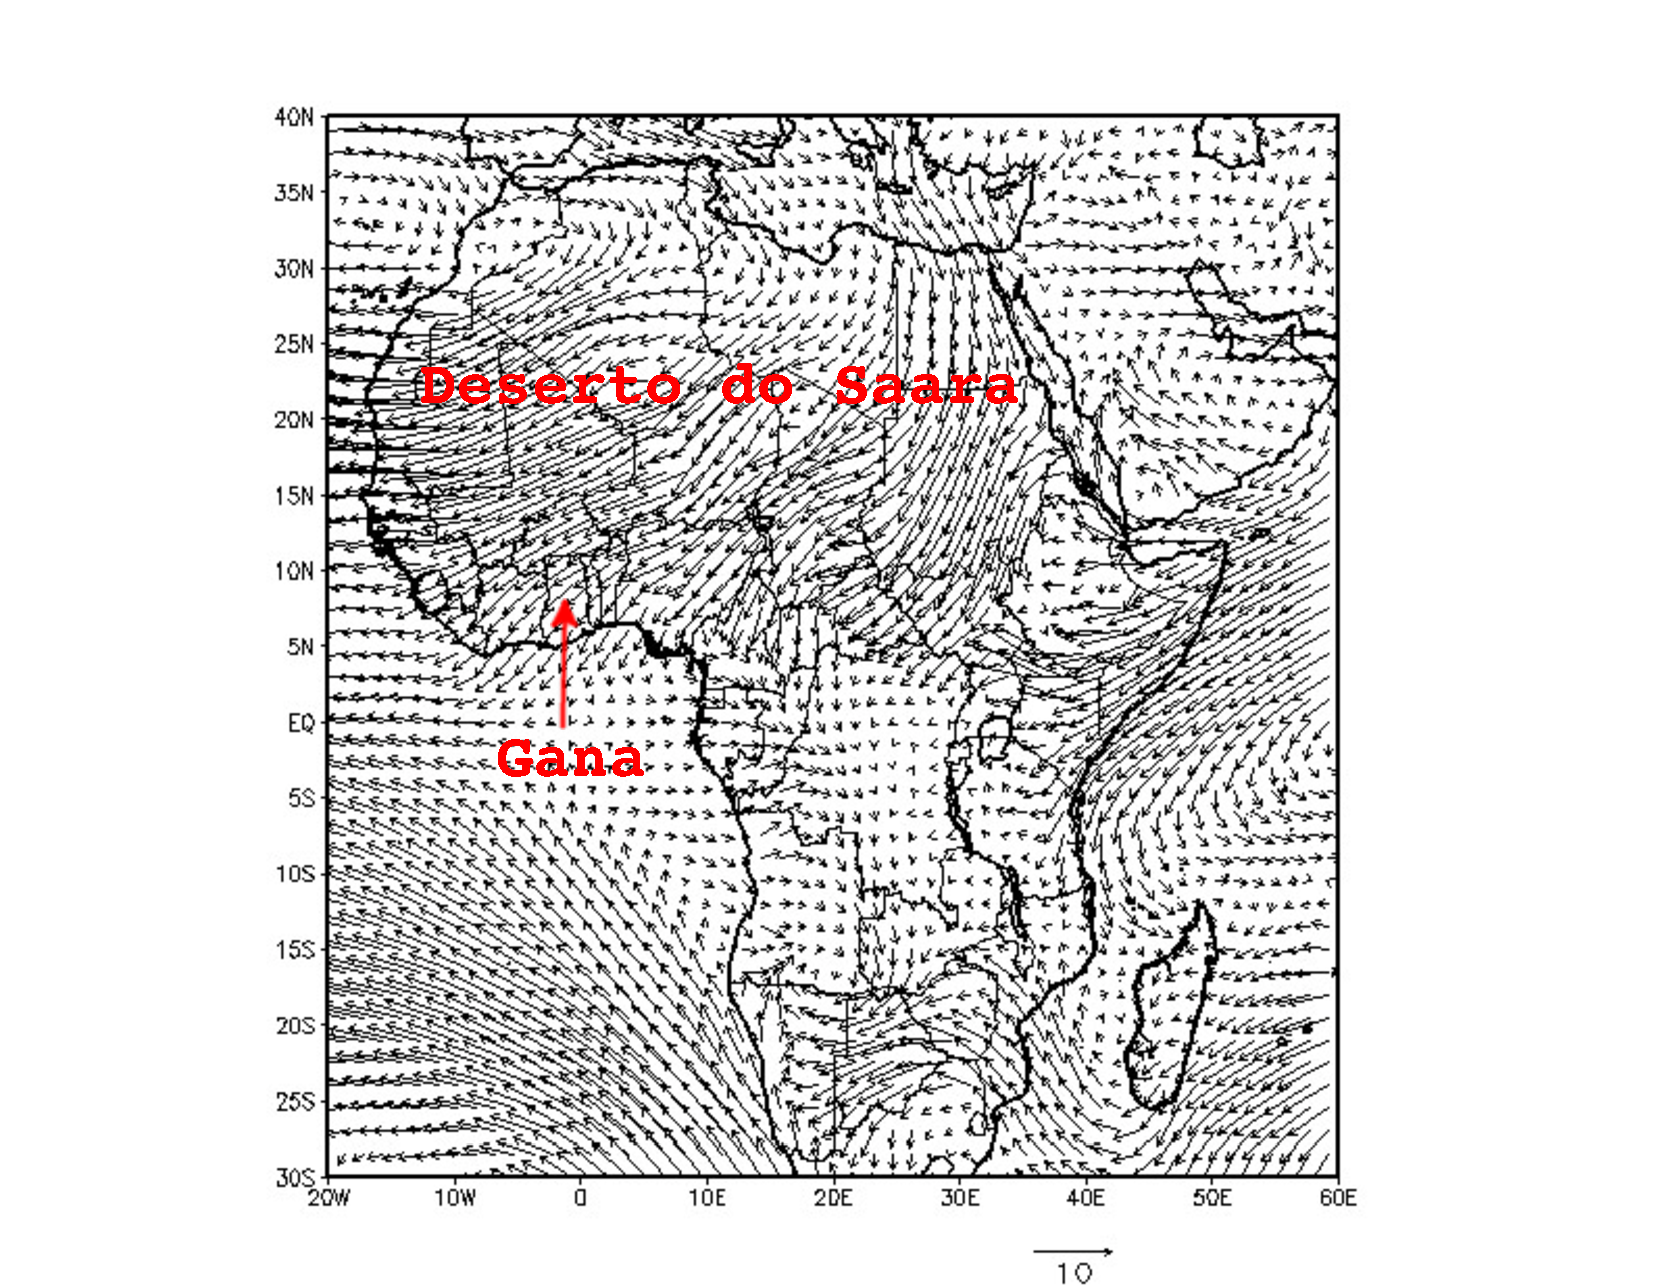
\includegraphics[width=\linewidth]{../../inputs/grads/gimp/875hPa/JAN_2008.pdf}
      \caption{Janeiro de 2008}
    \end{subfigure}
    \caption{Intensidade e direção do vento médio na altitude de 1000 metros 
             sobre o continente Africano. \label{fig:ECMWF1000}}
  \end{figure}
\end{frame}

%\begin{frame}
%  \frametitle{}
%    \input{../../outputs/loadings_RFsH.tex}
%\end{frame}

%\begin{frame}
%  \frametitle{}
%    \input{../../outputs/loadings_TFsH.tex}
%\end{frame}

%\begin{frame}
%  \frametitle{Impacto do Harmatã}
%  \begin{figure}[H]
%   \centering
%   \includegraphics[scale=0.30]{../../outputs/score_TIcH1.pdf}
%    \includegraphics[scale=0.30]{../../../outputs/score_TIcH3.pdf}
%  \end{figure}
%   Score para fator que representa \textcolor{red}{solo/Harmatã} 
%   e \textcolor{red}{Queima de Biomassa}, respectivamente.
%\end{frame}

%\begin{frame}
%    Perfil e Contribuição das fontes(\%) no bairro para $MP_{2.5}$:
%    \begin{tiny}
%      \input{../../outputs/RFsH_profiles_percent_species.tex}
%      \input{../../outputs/RFsH_contribution.tex}
%    \end{tiny}
%\end{frame}

%\begin{frame}
%    Perfil e Contribuição das fontes(\%) na Avenida para $MP_{2.5}$:
%    \begin{tiny}
%      \input{../../outputs/TFsH_profiles_percent_species.tex}
%      \input{../../outputs/TFsH_contribution.tex}
%    \end{tiny}
%\end{frame}


\begin{frame}
  \frametitle{}
  \begin{figure}[H]
    \centering
    \includegraphics[width=0.9\textwidth]{../../outputs/BC_monarch71.pdf}
    \caption{Calibração do refletômetro do LAPAt em 2007 usando alvos padrões M71.
           \label{fig:monarch71}}
  \end{figure}
\end{frame}


\begin{frame}
  \frametitle{}
  \begin{figure}[H]
  	\centering
  	\includegraphics[width=0.7\linewidth]{../../outputs/BC_cetesb.pdf}
  	\caption{Reflêtancia e pesagem dos padrões produzidos na CETESB com BC 
                   de referência ASTM-N762. \label{fig:bc_cetesb}}
  \end{figure}
\end{frame}


\begin{frame}
  \frametitle{}
  \begin{figure}[H]
    \centering
    \includegraphics[width=0.5\linewidth]{../../outputs/JQ_TOT_Refletancia.pdf}
    \caption{Intercalibração TOT e Reflêtancia para amostragem paralela no 
             túnel Jânio Quadros. \label{table:interJQ}}
  \end{figure}
\end{frame}


\begin{frame}
  \frametitle{}
  \begin{figure}[H]
    \centering
    \begin{minipage}[b]{0.5\linewidth}
      \includegraphics[width=\textwidth]{../../outputs/BC_janio_quadros.pdf}
      \caption{Comparação da massa de BC das amostras do túnel Jânio Quadros 
               calculada usando calibração por TOT versus calibração a partir dos 
               alvos padrões produzidos na CETESB. \label{fig:JQ}}
    \end{minipage}
    \hspace{0.5cm}
    \begin{minipage}[b]{0.45\linewidth}
      \begin{small}
        \input{../../outputs/BC_janio_quadros.tex}
      \end{small}
      \captionof{table}{Comparação da massa de BC das amostras do túnel Jânio Quadros 
               calculada usando calibração por TOT(1) versus calibração a partir dos 
               alvos padrões produzidos na CETESB(2). \label{table:JQ}}
    \end{minipage}
  \end{figure}
\end{frame}


\begin{frame}
  \frametitle{}
  \begin{figure}[H]
  	\begin{center}
  		\includegraphics[width=0.9\textwidth]{../../outputs/Gana_TOT_Refletancia.pdf}
  		\caption{Intercalibração entre TOT e refletância em Acra. \label{fig:interGanaBC}}
  	\end{center}
  \end{figure}
\end{frame}

\begin{frame}
  \frametitle{}
  \begin{figure}[H]
  	\centering
  	\begin{subfigure}[b]{0.43\linewidth}
  		\includegraphics[width=\linewidth]{../../outputs/BC_compara_calibs.pdf}
  		\caption{Acra \label{fig:razaoTOTM71}}
  	\end{subfigure}
  		\hspace{0.3cm}
  	\begin{subfigure}[b]{0.43\linewidth}
  		\includegraphics[width=\linewidth]{../../outputs/BC_compara_calibs_recife.pdf}
  		\caption{Recife \label{fig:BC_compara_recife}}
  	\end{subfigure}%
  
  	\caption{Razão dos valores de BC medidos por refletância e calibrados por 
  		TOT e M71 para Recife e Acra. \label{fig:BC_compara}}
  \end{figure}
\end{frame}


\begin{frame}
  \frametitle{}
\end{frame}



\begin{frame}
  \frametitle{}
\end{frame}


\begin{frame}
  \frametitle{}
\end{frame}


\begin{frame}
  \frametitle{}
\end{frame}



\begin{frame}
  \frametitle{}
\end{frame}


\begin{frame}
  \frametitle{}
\end{frame}



\begin{frame}
  \frametitle{}
\end{frame}


\begin{frame}
  \frametitle{}
\end{frame}

